%%%%%%%%%%%%%%%%%%%%%%%%%%%%%%%%%%%%%%%%%
% Journal Article
% LaTeX Template
% Version 1.3 (9/9/13)
%
% This template has been downloaded from:
% http://www.LaTeXTemplates.com
%
% Original author:
% Frits Wenneker (http://www.howtotex.com)
%
% License:
% CC BY-NC-SA 3.0 (http://creativecommons.org/licenses/by-nc-sa/3.0/)
%
%%%%%%%%%%%%%%%%%%%%%%%%%%%%%%%%%%%%%%%%%
%----------------------------------------------------------------------------------------
%       PACKAGES AND OTHER DOCUMENT CONFIGURATIONS
%----------------------------------------------------------------------------------------
\documentclass[paper=letter, fontsize=10pt]{article}
\usepackage[english]{babel} % English language/hyphenation
\usepackage{amsmath,amsfonts,amsthm} % Math packages
\usepackage[utf8]{inputenc}
\usepackage{blindtext, subcaption, caption, graphicx, float, hyperref, tikz, pgfplots}
% float: Required for tables and figures in the multi-column environment - they need to be placed in specific locations with the [H] (e.g. \begin{table}[H])
% Hyperref: For hyperlinks in the PDF
\usepackage[sc]{mathpazo} % Use the Palatino font
\usepackage[T1]{fontenc} % Use 8-bit encoding that has 256 glyphs
\linespread{1.05} % Line spacing - Palatino needs more space between lines
\usepackage{microtype} % Slightly tweak font spacing for aesthetics
\usepackage[hmarginratio=1:1,top=32mm,columnsep=20pt]{geometry} % Document margins
\usepackage{multicol} % Used for the two-column layout of the document
%\usepackage[hang, small,labelfont=bf,up,textfont=it,up]{caption} % Custom captions under/above floats in tables or figures
\usepackage{booktabs} % Horizontal rules in tables
\usepackage{lettrine} % The lettrine is the first enlarged letter at the beginning of the text
\usepackage{paralist} % Used for the compactitem environment which makes bullet points with less space between them
\usepackage{abstract} % Allows abstract customization
\renewcommand{\abstractnamefont}{\normalfont\bfseries} % Set the "Abstract" text to bold
\renewcommand{\abstracttextfont}{\normalfont\small\itshape} % Set the abstract itself to small italic text
\usepackage{titlesec} % Allows customization of titles

\renewcommand\thesection{\Roman{section}} % Roman numerals for the sections
\renewcommand\thesubsection{\Roman{subsection}} % Roman numerals for subsections

\titleformat{\section}[block]{\large\scshape\centering}{\thesection.}{1em}{} % Change the look of the section titles
\titleformat{\subsection}[block]{\large}{\thesubsection.}{1em}{} % Change the look of the section titles
\newcommand{\horrule}[1]{\rule{\linewidth}{#1}} % Create horizontal rule command with 1 argument of height
\usepackage{fancyhdr} % Headers and footers
\pagestyle{fancy} % All pages have headers and footers
\fancyhead{} % Blank out the default header
\fancyfoot{} % Blank out the default footer

\fancyhead[C]{University of Southern Denmark $\bullet$ RM-UAST $\bullet$ Spring 2017 $\bullet$ Group 5 } % Custom header text

\fancyfoot[RO,LE]{\thepage} % Custom footer text
%----------------------------------------------------------------------------------------
%       TITLE SECTION
%----------------------------------------------------------------------------------------
\title{\vspace{-15mm}\fontsize{24pt}{10pt}\selectfont\textbf{Module Five }} % Article title
\author{
\large
{\textsc{}}\\[2mm]
{\textsc{Henrik Frank, hefra13@student.sdu.dk }}\\[2mm]
{\textsc{Christian Arentsen, chare13@student.sdu.dk }}\\[2mm]
{\textsc{Vasileios Karvouniaris, vakar15@student.sdu.dk }}\\[2mm]
{\textsc{Asbjørn Schou Müller, asmul10@student.sdu.dk }}
%\thanks{A thank you or further information}\\ % Your name
%\normalsize \href{mailto:marco.torres.810@gmail.com}{marco.torres.810@gmail.com}\\[2mm] % Your email address
}
\date{}

%----------------------------------------------------------------------------------------
\begin{document}
\maketitle % Insert title
\thispagestyle{fancy} % All pages have headers and footers

\section{Attitude sensing using accelerometers}

The purpose of this exercise is to learn how to calculate the aircraft orientation based on these linear accelerations. The exercise is based on data sampled from a SparkFun Razor Inertial Measurement Unit (IMU) (figure \ref{fig:razor}). 

\subsection{Calculate pitch angle}
The file \texttt{imu\_razor\_data\_pitch\_45deg.txt} contains a dataset that was sampled while the IMU was tilted forwards and back

Use the Python script \texttt{imu\_exercise.py} to perform a calculation of the pitch angle based on the accelerometer values. Use the equation 28 in the document \textit{Tilt Sensing Using a Three-Axis Accelerometer.pdf}

Observe that the plot shows the expected output based on the description of the dataset.

\paragraph{Results}
Looking at the plot, figure~\ref{fig:ex1_plot}, we see the pitch angle as a function of time, and a pitch angle of roughly up to 55 degrees pitch.

\begin{figure}[h!]
\centering
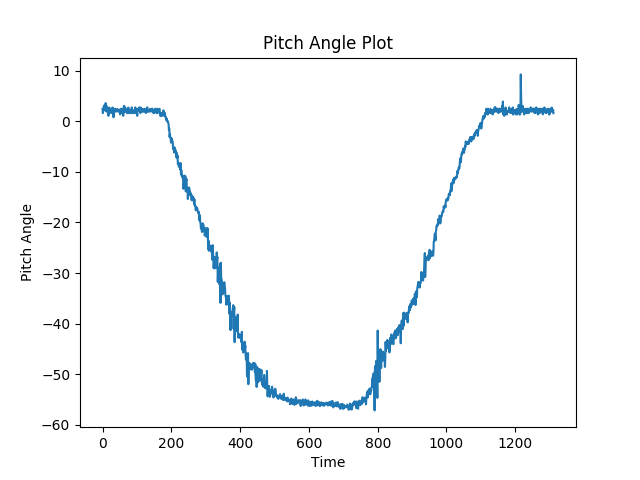
\includegraphics[scale=.65]{Figures/ex1_pitch_angle}
\caption{Figure of a pitch up to roughly 55 degrees}
\label{fig:ex1_plot}
\end{figure}

\subsection{Calculate roll angle}
The file \texttt{imu\_razor\_data\_roll\_45deg.txt} contains a dataset that was sampled while the IMU was tilted to the side.

Use the Python script \texttt{imu\_exercise.py} to perform a calculation of the roll angle based on the accelerometer values. Use the equation 29 in the document \textit{Tilt Sensing Using a Three-Axis Accelerometer.pdf}

Observe that the plot shows the expected output based on the description of the dataset.


\paragraph{Results}
Looking at the plot, figure~\ref{fig:ex1_roll_plot}, we see the roll angle as a function of time, which is consistent with shifting sides, rolling to left and right afterwards.

\begin{figure}[h!]
\centering
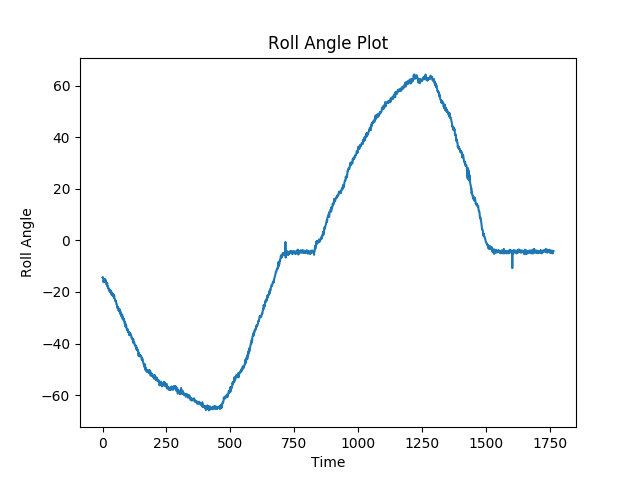
\includegraphics[scale=.65]{Figures/ex1_roll_angle}
\caption{Plot of rolling from side to side}
\label{fig:ex1_roll_plot}
\end{figure}

\subsection{Accelerometer noise}

The file \texttt{imu\_razor\_data\_static.txt} contains a dataset that was sampled for approx 60 seconds while the IMU was held static on a reasonably level surface.

Using the same calculations as in 1. and 2. plot the pitch and roll angles based on this dataset.

\begin{figure}[h!]
\centering
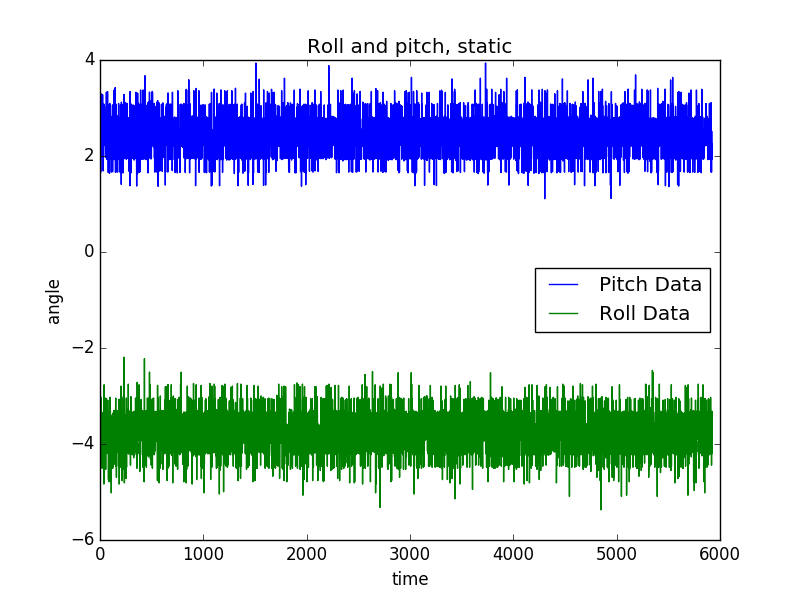
\includegraphics[scale=.5]{Figures/ex1_static}
\caption{Plot both roll and pitch in static position}
\label{fig:ex1_static_plot}
\end{figure}

Do the calculated angles show any significant noise or bias? Yes, in figure~\ref{fig:ex1_plot} shows a jump around 800th millisecond, and same goes for figure~\ref{fig:ex1_roll_plot} at around 700 and again at 1600. The static plots in fig~\ref{fig:ex1_static_plot} shows a general bias of $+/-$ 2 degrees.

How could this be mitigated? Using filtering, such as a Kalman filter.


\subsection{Low-pass filtering}

Try adding a low-pass filter and see if you can reduce the noise.
How much delay do you then add to the estimation of the pitch and roll angle?
Is this acceptable given the update velocity of the stability controller?

\begin{figure}[h!]
\centering
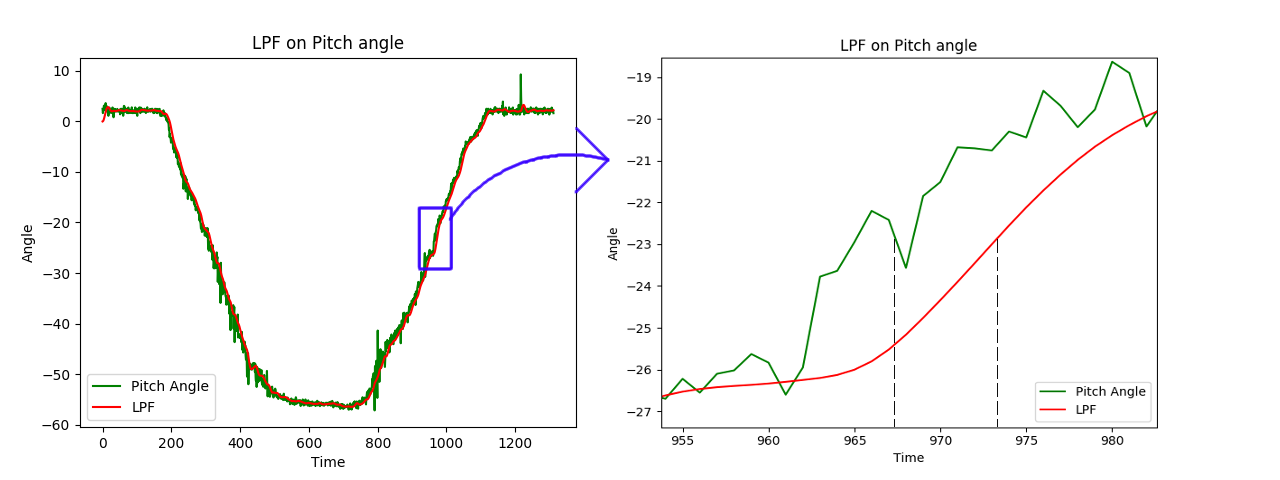
\includegraphics[scale=.5]{Figures/ex1_4_pitch_with_filter}
\caption{LPF on Pitch angle data}
\label{fig:ex1_lpf_on_pitch}
\end{figure}

\paragraph{Results} 
As seen in figure~\ref{fig:ex1_lpf_on_pitch}, implementing a low pass filter can smoothen a graph, yet, if one looks closer to the filtered graph, the right hand side of figure~\ref{fig:ex1_lpf_on_pitch}, on can clearly see that that using the low pass filter, the information returned by the filter is delayed but only a little, however, this has huge impact on flight controlling. 

\subsection{Limitations of Euler angles}

The equations 28 and 29 used above are not able to describe all states of orientation, this is well known as \textit{Gimbal lock}. Which particular orientations may cause problems?

\subsection{Extra: Quaternions}

Implement a pitch and roll estimation ot suffering from the gimbal lock limitations using Quaternions.


\section{Gyro measurements}

The purpose of this exercise is to learn how to integrate the angular velocities measured by a gyro to obtain a relative measure of the angle about that axis.

The exercise is based on data sampled from a SparkFun Razor Inertial Measurement Unit (IMU) (figure \ref{fig:razor}) and a VectorNav VN-100 IMU (figure \ref{fig:vn100}). 
\begin{figure}
\centering
\begin{minipage}{.5\textwidth}
	\centering
	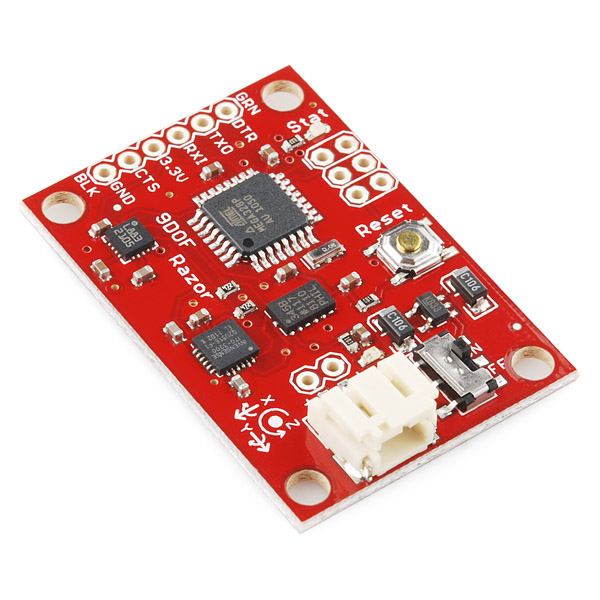
\includegraphics[width=.4\linewidth]{images/sparkfun_razor.jpg}
	\caption{\textit{SparkFun Razor IMU.}}
	\label{fig:razor}
\end{minipage}%
\begin{minipage}{.5\textwidth}
	\centering
	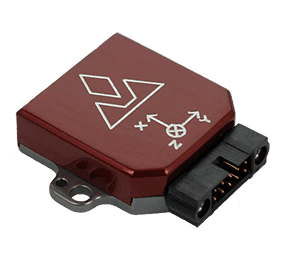
\includegraphics[width=.4\linewidth]{images/vn-100-rugged.png}
	\caption{\textit{VectorNav VN-100 IMU.}}
	\label{fig:vn100}
\end{minipage}
\end{figure}


\subsection{Calculating relative angle}
The file \texttt{imu\_razor\_data\_yaw\_90deg.txt} contains a dataset that was sampled while the IMU was turned $90\,^{\circ}$ clockwise, then the IMU was turned $90\,^{\circ}$ counter-clockwise. 

Use the Python script \texttt{imu\_exercise.py} to perform a numerical integration of the angular velocity about the z-axis $\omega_z$ to obtain a measure of the relative angle. Use the actual time since the previous received angular velocity for the integration.

Observe that the plot shows the expected output based on the description of the dataset.

\paragraph{Results} 
The graph in figure~\ref{fig:ex2_gyro_zaxis} shows how the IMU moves to the right for approximately 90 degrees, and then turns back to original position.  
\begin{figure}
	\centering
	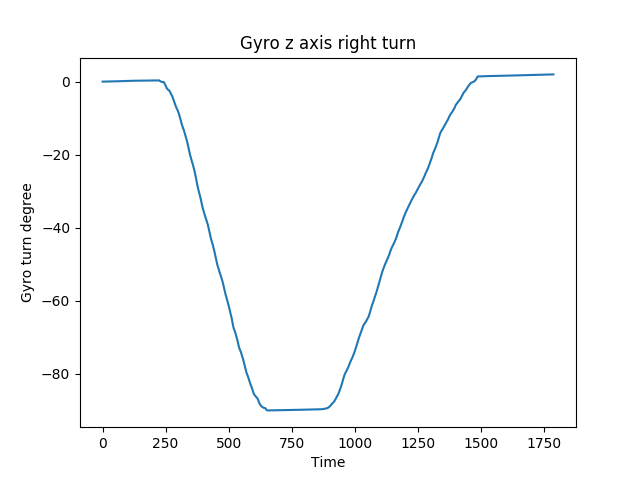
\includegraphics[scale=0.65]{Figures/ex2_gyro_zaxis}
	\caption{Plot showing IMU turning right 90 degrees, \\and back to original position}
	\label{fig:ex2_gyro_zaxis}
\end{figure}

\subsection{Static data}
The file \texttt{imu\_razor\_data\_static.txt} contains a dataset that was sampled for approx 60 seconds while the IMU was held static on a reasonably level surface.

Perform the same numerical integration of the angular velocity and observe the result.

\paragraph{Results} The plot in figure~\ref{fig:ex2_gyro_static} shows how the gyro, though in a static position, has a little positive drift value, resulting in a gain of around 2.5 degrees in just 6 minutes. Should we rely on gyro alone, this is a rather high bias.

\begin{figure}
	\centering
	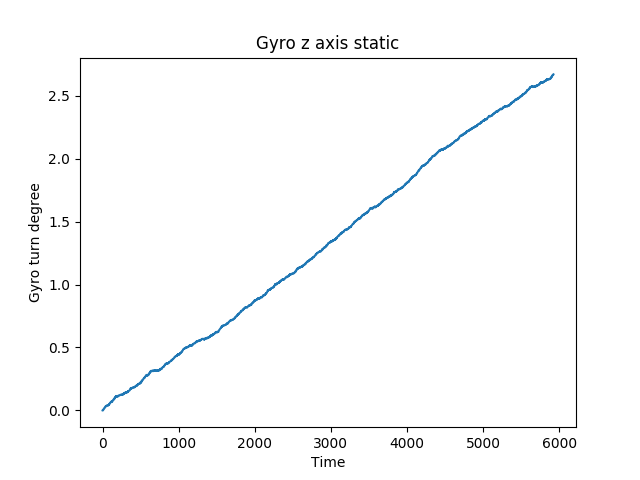
\includegraphics[scale=0.65]{Figures/ex2_gyro_static}
	\caption{Plot showing IMU in static position}
	\label{fig:ex2_gyro_static}
\end{figure}


\subsection{Observing bias}
The output from the integration shows that the relative angle is drifting. The drift is the visible effect of a bias on the angular velocity.

Try to estimate the bias and subtract it before integrating.  

\paragraph{Results}
The drifting bias is around 0.5 degree a minute. More accurately 0.0008 per step.

\subsection{Bias sources}
Consider the potential sources of noise and bias for a gyro?

\paragraph{Results} Bias error tends to vary, both with temperature and over time. The bias error of a gyro is due to a number of components:
\begin{itemize}
\item calibration errors
\item switch-on to switch-on
\item bias drift
\item efects of shock (g level)\cite{sensorwiki}.
\end{itemize}
For reducing drift bias, one uses a  warm-up period.


\subsection{Extra: Integration using average time}

Perform a similar numerical integration but this time use a calculated average time between updates in the file.

Consider why there is a difference and what gives the most accurate result?

\subsection{Extra: Record more datasets}

Use the Python script \texttt{nmea\_data\_logger.py} and an IMU to record other datasets. 


\section{Kalman filter}

The purpose of this exercise is to learn how a Kalman filter will improve the attitude estimation using the accelerometers and gyros as input.

\subsection{Implementing a scalar Kalman filter}

Implement a scalar Kalman filter estimating the Pitch angle in the Python script \texttt{imu\_exercise\_kalman.py}. To do this you must add the calculation of pitch and roll from the accelerometers and then the gyro relative angles from the previous exercises.

Please notice that within the script two sections are clearly marked \textit{Insert initialize code below} and \textit{Insert loop code below}. You do not need to change anything in the file outside these sections.

\paragraph{Results}
We have had some issues with implementing the kalman filter, see progress at GitHub.

%\pagebreak

\bibliographystyle{plain}
%https://en.wikipedia.org/wiki/Line-of-sight_propagation
\bibliography{bibfile}
%----------------------------------------------------------------------------------------
%\end{multicols}
\end{document}
